% Cahier d'analyse - Gestion Agricole Intelligente
\documentclass[12pt,a4paper]{report}
\usepackage[T1]{fontenc}
\usepackage[utf8]{inputenc}
\usepackage[french]{babel}
\usepackage{lmodern}
\usepackage{geometry}
\usepackage{graphicx}
\usepackage{hyperref}
\usepackage{caption}
\usepackage{longtable}
\usepackage{array}
\usepackage{float}
\usepackage[table]{xcolor}
\usepackage{booktabs}
\usepackage{fancyhdr}
\geometry{top=2.5cm,bottom=2.5cm,left=2.5cm,right=2.5cm}
\setlength{\LTleft}{0pt}
\setlength{\LTright}{0pt}
\setlength{\tabcolsep}{6pt}
\renewcommand{\arraystretch}{1.2}
\setcounter{secnumdepth}{3}
\setcounter{tocdepth}{3}
\pagestyle{fancy}
\fancyhf{}
\fancyfoot[C]{\thepage}
\renewcommand{\headrulewidth}{0pt}
\renewcommand{\footrulewidth}{0pt}
\providecommand{\tightlist}{\setlength{\itemsep}{0pt}\setlength{\parskip}{0pt}}
\begin{document}
\begin{titlepage}
  \begin{minipage}[t]{0.48\textwidth}
    \raggedright
    {\small UNIVERSITÉ DE YAOUNDÉ I}\\[0.2cm]
    {\small **********}\\[0.2cm]
    {\small ÉCOLE NATIONALE SUPÉRIEURE POLYTECHNIQUE DE YAOUNDÉ}\\[0.2cm]
    {\small **********}\\[0.2cm]
    {\small DÉPARTEMENT DU GÉNIE}\\
    {\small INFORMATIQUE}\\[0.2cm]
    {\small **********}\\[0.2cm]
    {\small ARTS NUMÉRIQUES}
  \end{minipage}%
  \hfill
  \begin{minipage}[t]{0.48\textwidth}
    \raggedleft
    {\small THE UNIVERSITY OF YAOUNDE I}\\[0.2cm]
    {\small **********}\\[0.2cm]
    {\small NATIONAL ADVANCED SCHOOL OF ENGINEERING OF YAOUNDE}\\[0.2cm]
    {\small **********}\\[0.2cm]
    {\small DEPARTMENT OF COMPUTER}\\
    {\small ENGINEERING}\\[0.2cm]
    {\small **********}\\[0.2cm]
    {\small DIGITAL ARTS}
  \end{minipage}

  \begin{center}
    
\includegraphics[width=0.28\textwidth]{images/logo-enspy.png}\\[1cm]

    {\LARGE \textbf{Cahier d'analyse}}\\[0.6cm]
    {\Huge \textbf{Analyse fonctionnelle d'une application de gestion agricole intelligente}}\\[1cm]

    {\large \textit{Genie Logiciel I}}\\[0.8cm]

    {\large \textbf{Rédaction}}\\[0.3cm]
    {\large Tambou Djomou Franck Donald 23P732}\\
    {\large Kanmo Ngamini Bella Rinda 22P008}\\[0.8cm]

    {\large Encadrant : Dr Kungne}\\[0.4cm]
    {\large Date : juin 2026}\\[0.4cm]

    {\small \textit{Ce document présente l'analyse fonctionnelle et les cas d'utilisation du projet.}}
  \end{center}

  \vfill
  \thispagestyle{empty}
\end{titlepage}
\pagenumbering{roman}
\tableofcontents
\listoffigures
\clearpage
\pagenumbering{arabic}
\hypertarget{chapitre-1-introduction}{%
\chapter{INTRODUCTION}\label{chapitre-1-introduction}}

\hypertarget{contexte-de-lanalyse}{%
\section{Contexte de l'Analyse}\label{contexte-de-lanalyse}}

Après l'identification des besoins et la définition des exigences dans
le cahier des charges, il est nécessaire de procéder à une analyse
détaillée du système à développer.

L'analyse constitue une étape essentielle du cycle de développement
logiciel. Elle permet de comprendre les besoins des utilisateurs,
d'identifier les services attendus du système et de définir les
interactions entre les différents acteurs et le système.

Dans le cadre du présent projet, l'analyse porte sur une application de
gestion agricole intelligente destinée à assurer le suivi des cultures,
la prédiction des rendements et la fourniture de recommandations
agronomiques.

\hypertarget{objectif-de-lanalyse}{%
\section{Objectif de l'Analyse}\label{objectif-de-lanalyse}}

L'objectif principal de cette phase est de décrire le comportement
attendu du système indépendamment de toute considération technique liée
à son implémentation.

Cette analyse vise notamment à :

\begin{itemize}
\item
  \begin{quote}
  identifier les acteurs du système ;
  \end{quote}
\item
  \begin{quote}
  identifier les services attendus ;
  \end{quote}
\item
  \begin{quote}
  modéliser les interactions entre les acteurs et le système ;
  \end{quote}
\item
  \begin{quote}
  décrire les cas d'utilisation ;
  \end{quote}
\item
  \begin{quote}
  préparer la phase de conception.
  \end{quote}
\end{itemize}

\hypertarget{muxe9thodologie-danalyse}{%
\section{Méthodologie d'Analyse}\label{muxe9thodologie-danalyse}}

L'analyse est réalisée selon une approche orientée cas d'utilisation.

Le système est considéré comme une boîte noire et seules les
fonctionnalités visibles par les utilisateurs sont prises en compte.

Cette démarche permet de répondre à la question « Que doit faire le
système ? » sans s'intéresser à la manière dont ces fonctionnalités
seront implémentées.

Les modèles UML utilisés dans cette phase sont :

\begin{itemize}
\item
  \begin{quote}
  le diagramme de cas d'utilisation ;
  \end{quote}
\item
  \begin{quote}
  les descriptions détaillées des cas d'utilisation ;
  \end{quote}
\item
  \begin{quote}
  les diagrammes de séquence système.
  \end{quote}
\end{itemize}

\hypertarget{chapitre-2-vision-produit}{%
\chapter{VISION PRODUIT}\label{chapitre-2-vision-produit}}

\hypertarget{vision-produit}{%
\section{Vision Produit}\label{vision-produit}}

L'application de gestion agricole intelligente permettra aux acteurs du
secteur agricole de suivre l'évolution de leurs cultures, d'obtenir des
estimations de rendement et de bénéficier de recommandations
agronomiques adaptées afin d'améliorer la gestion de leurs activités
agricoles et leur prise de décision.

Le système centralisera les informations relatives aux cultures et
offrira des services d'assistance permettant d'optimiser le suivi et la
productivité agricole.

\hypertarget{justification-de-la-vision-produit}{%
\section{Justification de la Vision
Produit}\label{justification-de-la-vision-produit}}

La vision produit constitue le point de référence de l'ensemble du
projet. Elle exprime la finalité du système et oriente les décisions
prises durant les phases d'analyse, de conception et d'implémentation.

Dans le cadre de ce projet, la vision retenue met l'accent sur trois
besoins majeurs identifiés lors de l'étude préalable :

\begin{itemize}
\item
  \begin{quote}
  le suivi des cultures ;
  \end{quote}
\item
  \begin{quote}
  la prédiction des rendements ;
  \end{quote}
\item
  \begin{quote}
  les recommandations agronomiques.
  \end{quote}
\end{itemize}

Ces trois axes correspondent aux objectifs principaux du système et
serviront de guide pour l'identification des fonctionnalités et des cas
d'utilisation.

\hypertarget{objectifs-du-systuxe8me}{%
\section{Objectifs du Système}\label{objectifs-du-systuxe8me}}

Afin de concrétiser la vision produit, le système devra permettre :

\begin{itemize}
\item
  \begin{quote}
  la gestion des informations relatives aux cultures ;
  \end{quote}
\item
  \begin{quote}
  le suivi de l'évolution des cultures ;
  \end{quote}
\item
  \begin{quote}
  l'enregistrement et la consultation des observations agricoles ;
  \end{quote}
\item
  \begin{quote}
  l'obtention de prédictions de rendement ;
  \end{quote}
\item
  \begin{quote}
  l'obtention de recommandations agronomiques ;
  \end{quote}
\item
  \begin{quote}
  la gestion sécurisée des utilisateurs ;
  \end{quote}
\item
  \begin{quote}
  l'administration générale de la plateforme.
  \end{quote}
\end{itemize}

\hypertarget{puxe9rimuxe8tre-fonctionnel-de-lanalyse}{%
\section{Périmètre Fonctionnel de
l'Analyse}\label{puxe9rimuxe8tre-fonctionnel-de-lanalyse}}

L'analyse porte uniquement sur les fonctionnalités définies dans le
cahier des charges.

Sont inclus dans le périmètre :

\begin{itemize}
\item
  \begin{quote}
  la gestion des cultures ;
  \end{quote}
\item
  \begin{quote}
  le suivi des cultures ;
  \end{quote}
\item
  \begin{quote}
  la prédiction des rendements ;
  \end{quote}
\item
  \begin{quote}
  les recommandations agronomiques ;
  \end{quote}
\item
  \begin{quote}
  la gestion des utilisateurs ;
  \end{quote}
\item
  \begin{quote}
  l'administration du système.
  \end{quote}
\end{itemize}

Ne font pas partie du périmètre :

\begin{itemize}
\item
  \begin{quote}
  la gestion financière des exploitations ;
  \end{quote}
\item
  \begin{quote}
  la commercialisation des produits agricoles ;
  \end{quote}
\item
  \begin{quote}
  la gestion du matériel agricole ;
  \end{quote}
\item
  \begin{quote}
  les paiements électroniques ;
  \end{quote}
\item
  \begin{quote}
  l'intégration de capteurs IoT ;
  \end{quote}
\item
  \begin{quote}
  les données météorologiques en temps réel.
  \end{quote}
\end{itemize}

Cette limitation permet de maintenir la cohérence avec le cahier des
charges et de respecter les contraintes temporelles du projet.

\hypertarget{chapitre-3-identification-des-acteurs}{%
\chapter{IDENTIFICATION DES
ACTEURS}\label{chapitre-3-identification-des-acteurs}}

\hypertarget{introduction}{%
\section{Introduction}\label{introduction}}

Les acteurs représentent les entités externes qui interagissent avec le
système afin d'obtenir un service ou de fournir des informations.

L'identification des acteurs constitue une étape essentielle de
l'analyse puisqu'elle permet de déterminer les différents utilisateurs
du système ainsi que leurs responsabilités respectives.

Pour l'application de gestion agricole intelligente, quatre acteurs
principaux ont été identifiés.

\hypertarget{agriculteur}{%
\section{Agriculteur}\label{agriculteur}}

L'agriculteur est l'acteur principal du système.

Il utilise l'application pour assurer la gestion et le suivi de ses
cultures tout au long de leur cycle de production.

\hypertarget{responsabilituxe9s}{%
\subsection{Responsabilités}\label{responsabilituxe9s}}

L'agriculteur peut :

\begin{itemize}
\item
  \begin{quote}
  gérer les informations relatives aux cultures ;
  \end{quote}
\item
  \begin{quote}
  enregistrer des observations agricoles ;
  \end{quote}
\item
  \begin{quote}
  suivre l'évolution des cultures ;
  \end{quote}
\item
  \begin{quote}
  obtenir des prédictions de rendement ;
  \end{quote}
\item
  \begin{quote}
  obtenir des recommandations agronomiques.
  \end{quote}
\end{itemize}

L'agriculteur est le principal bénéficiaire des services fournis par le
système.

\hypertarget{agronome}{%
\section{Agronome}\label{agronome}}

L'agronome intervient comme expert agricole.

Son rôle consiste à analyser les informations relatives aux cultures et
à exploiter les résultats produits par le système.

\hypertarget{responsabilituxe9s-1}{%
\subsection{Responsabilités}\label{responsabilituxe9s-1}}

L'agronome peut :

\begin{itemize}
\item
  \begin{quote}
  consulter les informations relatives aux cultures ;
  \end{quote}
\item
  \begin{quote}
  suivre l'évolution des cultures ;
  \end{quote}
\item
  \begin{quote}
  consulter les prédictions de rendement ;
  \end{quote}
\item
  \begin{quote}
  consulter les recommandations agronomiques.
  \end{quote}
\end{itemize}

Il participe à l'interprétation des informations fournies par le
système.

\hypertarget{administrateur}{%
\section{Administrateur}\label{administrateur}}

L'administrateur est chargé de la gestion générale de la plateforme.

Il veille au bon fonctionnement du système et assure la gestion des
utilisateurs.

\hypertarget{responsabilituxe9s-2}{%
\subsection{Responsabilités}\label{responsabilituxe9s-2}}

L'administrateur peut :

\begin{itemize}
\item
  \begin{quote}
  gérer les comptes utilisateurs ;
  \end{quote}
\item
  \begin{quote}
  administrer les données du système ;
  \end{quote}
\item
  \begin{quote}
  superviser le fonctionnement général de l'application.
  \end{quote}
\end{itemize}

\hypertarget{service-de-pruxe9diction}{%
\section{Service de Prédiction}\label{service-de-pruxe9diction}}

Le service de prédiction constitue un acteur externe au système.

Il intervient lors de l'estimation des rendements agricoles.

\hypertarget{responsabilituxe9s-3}{%
\subsection{Responsabilités}\label{responsabilituxe9s-3}}

Le service de prédiction peut :

\begin{itemize}
\item
  \begin{quote}
  recevoir les informations nécessaires à l'analyse ;
  \end{quote}
\item
  \begin{quote}
  produire une estimation du rendement ;
  \end{quote}
\item
  \begin{quote}
  transmettre les résultats au système.
  \end{quote}
\end{itemize}

Cet acteur représente le mécanisme externe permettant la réalisation des
prédictions.

\hypertarget{synthuxe8se-des-acteurs}{%
\section{Synthèse des Acteurs}\label{synthuxe8se-des-acteurs}}

Le tableau suivant récapitule les acteurs identifiés.

\begin{longtable}{@{}p{0.20\linewidth}p{0.28\linewidth}p{0.48\linewidth}@{}}
\toprule
\rowcolors{2}{gray!10}{white}
\textbf{Acteur} & \textbf{Type} & \textbf{Rôle Principal} \\
\midrule
\endhead
Agriculteur & Acteur principal & Gestion et suivi des cultures \\
Agronome & Acteur secondaire & Analyse et consultation des informations
agricoles \\
Administrateur & Acteur secondaire & Administration de la plateforme \\
Service de Prédiction & Acteur externe & Fourniture des prédictions de
rendement \\
\bottomrule
\end{longtable}

L'ensemble de ces acteurs participera aux interactions modélisées dans
les cas d'utilisation du système.

\hypertarget{chapitre-4-identification-des-cas-dutilisation}{%
\chapter{IDENTIFICATION DES CAS
D'UTILISATION}\label{chapitre-4-identification-des-cas-dutilisation}}

\hypertarget{introduction-1}{%
\section{Introduction}\label{introduction-1}}

Les cas d'utilisation représentent les principaux services rendus par le
système aux acteurs identifiés lors de l'analyse.

Ils permettent de décrire les objectifs que les utilisateurs souhaitent
atteindre à travers leur interaction avec le système.

Dans le cadre de cette étude, les cas d'utilisation ont été définis à
partir des exigences fonctionnelles exprimées dans le cahier des charges
tout en conservant un niveau d'abstraction adapté à la phase d'analyse.

\hypertarget{cas-dutilisation-de-lagriculteur}{%
\section{Cas d'Utilisation de
l'Agriculteur}\label{cas-dutilisation-de-lagriculteur}}

L'agriculteur est l'acteur principal du système.

Les cas d'utilisation qui lui sont associés sont les suivants :

\hypertarget{cu1-sauthentifier}{%
\subsection{CU1 : S'authentifier}\label{cu1-sauthentifier}}

Permet à l'agriculteur d'accéder aux fonctionnalités du système.

\hypertarget{cu2-guxe9rer-les-cultures}{%
\subsection{CU2 : Gérer les cultures}\label{cu2-guxe9rer-les-cultures}}

Permet à l'agriculteur de gérer les informations relatives à ses
cultures.

Ce cas d'utilisation regroupe notamment :

\begin{itemize}
\item
  \begin{quote}
  l'enregistrement d'une culture ;
  \end{quote}
\item
  \begin{quote}
  la consultation d'une culture ;
  \end{quote}
\item
  \begin{quote}
  la modification d'une culture ;
  \end{quote}
\item
  \begin{quote}
  la suppression d'une culture.
  \end{quote}
\end{itemize}

\hypertarget{cu3-suivre-les-cultures}{%
\subsection{CU3 : Suivre les cultures}\label{cu3-suivre-les-cultures}}

Permet à l'agriculteur d'assurer le suivi de l'évolution de ses
cultures.

Ce cas d'utilisation couvre :

\begin{itemize}
\item
  \begin{quote}
  l'enregistrement des observations ;
  \end{quote}
\item
  \begin{quote}
  la consultation des observations ;
  \end{quote}
\item
  \begin{quote}
  le suivi de l'évolution des cultures.
  \end{quote}
\end{itemize}

\hypertarget{cu4-obtenir-une-pruxe9diction-de-rendement}{%
\subsection{CU4 : Obtenir une prédiction de
rendement}\label{cu4-obtenir-une-pruxe9diction-de-rendement}}

Permet à l'agriculteur d'obtenir une estimation du rendement attendu
pour une culture.

\hypertarget{cu5-obtenir-des-recommandations-agronomiques}{%
\subsection{CU5 : Obtenir des recommandations
agronomiques}\label{cu5-obtenir-des-recommandations-agronomiques}}

Permet à l'agriculteur de consulter des recommandations adaptées à la
situation observée.

\hypertarget{cas-dutilisation-de-lagronome}{%
\section{Cas d'Utilisation de
l'Agronome}\label{cas-dutilisation-de-lagronome}}

L'agronome intervient comme expert agricole.

Les cas d'utilisation qui lui sont associés sont :

\hypertarget{cu1-sauthentifier-1}{%
\subsection{CU1 : S'authentifier}\label{cu1-sauthentifier-1}}

\hypertarget{cu3-suivre-les-cultures-1}{%
\subsection{CU3 : Suivre les cultures}\label{cu3-suivre-les-cultures-1}}

\hypertarget{cu4-obtenir-une-pruxe9diction-de-rendement-1}{%
\subsection{CU4 : Obtenir une prédiction de
rendement}\label{cu4-obtenir-une-pruxe9diction-de-rendement-1}}

\hypertarget{cu5-obtenir-des-recommandations-agronomiques-1}{%
\subsection{CU5 : Obtenir des recommandations
agronomiques}\label{cu5-obtenir-des-recommandations-agronomiques-1}}

\hypertarget{cas-dutilisation-de-ladministrateur}{%
\section{Cas d'Utilisation de
l'Administrateur}\label{cas-dutilisation-de-ladministrateur}}

L'administrateur assure la gestion générale de la plateforme.

Les cas d'utilisation qui lui sont associés sont :

\hypertarget{cu1-sauthentifier-2}{%
\subsection{CU1 : S'authentifier}\label{cu1-sauthentifier-2}}

\hypertarget{cu6-guxe9rer-les-utilisateurs}{%
\subsection{CU6 : Gérer les
utilisateurs}\label{cu6-guxe9rer-les-utilisateurs}}

Permet la création, la modification, la consultation et la suppression
des comptes utilisateurs.

\hypertarget{cu7-administrer-le-systuxe8me}{%
\subsection{CU7 : Administrer le
système}\label{cu7-administrer-le-systuxe8me}}

Permet d'assurer le bon fonctionnement général de la plateforme.

\hypertarget{cas-dutilisation-du-service-de-pruxe9diction}{%
\section{Cas d'Utilisation du Service de
Prédiction}\label{cas-dutilisation-du-service-de-pruxe9diction}}

Le service de prédiction constitue un acteur externe.

Le cas d'utilisation associé est :

\hypertarget{cu8-fournir-une-pruxe9diction-de-rendement}{%
\subsection{CU8 : Fournir une prédiction de
rendement}\label{cu8-fournir-une-pruxe9diction-de-rendement}}

Permet de produire une estimation du rendement à partir des informations
transmises par le système.

\hypertarget{correspondance-entre-les-exigences-fonctionnelles-et-les-cas-dutilisation}{%
\section{Correspondance entre les Exigences Fonctionnelles et les
Cas
d'Utilisation}\label{correspondance-entre-les-exigences-fonctionnelles-et-les-cas-dutilisation}}

Les cas d'utilisation retenus sont directement issus des exigences
fonctionnelles définies dans le cahier des charges.

Afin de conserver un niveau d'abstraction adapté à la phase d'analyse,
plusieurs opérations détaillées ont été regroupées au sein de cas
d'utilisation métier plus généraux.

\begin{longtable}{@{}p{0.18\linewidth}p{0.78\linewidth}@{}}
\toprule
\rowcolors{2}{gray!10}{white}
\textbf{Exigences Fonctionnelles} & \textbf{Cas d'Utilisation Correspondant} \\
\midrule
\endhead
Créer un compte, consulter son profil, modifier son profil &
S'authentifier \\
Enregistrer une culture, consulter une culture, modifier une culture,
supprimer une culture & Gérer les cultures \\
Enregistrer une observation, consulter les observations, suivre
l'évolution d'une culture & Suivre les cultures \\
Demander une prédiction, consulter les résultats des prédictions &
Obtenir une prédiction de rendement \\
Générer une recommandation, consulter les recommandations & Obtenir des
recommandations agronomiques \\
Gérer les comptes utilisateurs & Gérer les utilisateurs \\
Administrer les données du système & Administrer le système \\
\bottomrule
\end{longtable}

Cette correspondance garantit la cohérence entre le cahier des charges
et le cahier d'analyse.

\hypertarget{synthuxe8se-des-cas-dutilisation}{%
\section{Synthèse des Cas
d'Utilisation}\label{synthuxe8se-des-cas-dutilisation}}

Les principaux cas d'utilisation du système sont :

\begin{itemize}
\item
  \begin{quote}
  CU1 : S'authentifier ;
  \end{quote}
\item
  \begin{quote}
  CU2 : Gérer les cultures ;
  \end{quote}
\item
  \begin{quote}
  CU3 : Suivre les cultures ;
  \end{quote}
\item
  \begin{quote}
  CU4 : Obtenir une prédiction de rendement ;
  \end{quote}
\item
  \begin{quote}
  CU5 : Obtenir des recommandations agronomiques ;
  \end{quote}
\item
  \begin{quote}
  CU6 : Gérer les utilisateurs ;
  \end{quote}
\item
  \begin{quote}
  CU7 : Administrer le système ;
  \end{quote}
\item
  \begin{quote}
  CU8 : Fournir une prédiction de rendement.
  \end{quote}
\end{itemize}

\hypertarget{chapitre-5-diagramme-de-cas-dutilisation}{%
\chapter{DIAGRAMME DE CAS
D'UTILISATION}\label{chapitre-5-diagramme-de-cas-dutilisation}}

\hypertarget{introduction-2}{%
\section{Introduction}\label{introduction-2}}

Le diagramme de cas d'utilisation permet de représenter les interactions
entre les acteurs et les services offerts par le système.

Il fournit une vue globale des fonctionnalités accessibles aux
différents utilisateurs tout en mettant en évidence les relations
existantes entre les cas d'utilisation.

Le diagramme présenté dans cette étude est élaboré à partir des acteurs
et des cas d'utilisation identifiés précédemment.

\hypertarget{acteurs-du-diagramme}{%
\section{Acteurs du Diagramme}\label{acteurs-du-diagramme}}

Les acteurs intervenant dans le système sont :

\begin{itemize}
\item
  \begin{quote}
  Agriculteur ;
  \end{quote}
\item
  \begin{quote}
  Agronome ;
  \end{quote}
\item
  \begin{quote}
  Administrateur ;
  \end{quote}
\item
  \begin{quote}
  Service de Prédiction.
  \end{quote}
\end{itemize}

\hypertarget{cas-dutilisation-du-diagramme}{%
\section{Cas d'Utilisation du
Diagramme}\label{cas-dutilisation-du-diagramme}}

Les principaux cas d'utilisation retenus sont :

\begin{itemize}
\item
  \begin{quote}
  CU1 : S'authentifier ;
  \end{quote}
\item
  \begin{quote}
  CU2 : Gérer les cultures ;
  \end{quote}
\item
  \begin{quote}
  CU3 : Suivre les cultures ;
  \end{quote}
\item
  \begin{quote}
  CU4 : Obtenir une prédiction de rendement ;
  \end{quote}
\item
  \begin{quote}
  CU5 : Obtenir des recommandations agronomiques ;
  \end{quote}
\item
  \begin{quote}
  CU6 : Gérer les utilisateurs ;
  \end{quote}
\item
  \begin{quote}
  CU7 : Administrer le système ;
  \end{quote}
\item
  \begin{quote}
  CU8 : Fournir une prédiction de rendement.
  \end{quote}
\end{itemize}

\hypertarget{relations-du-diagramme}{%
\section{Relations du Diagramme}\label{relations-du-diagramme}}

\hypertarget{relations-dassociation}{%
\subsection{Relations d'Association}\label{relations-dassociation}}

Les associations entre acteurs et cas d'utilisation sont les suivantes :

\hypertarget{agriculteur-1}{%
\subsubsection{Agriculteur}\label{agriculteur-1}}

\begin{itemize}
\item
  \begin{quote}
  S'authentifier ;
  \end{quote}
\item
  \begin{quote}
  Gérer les cultures ;
  \end{quote}
\item
  \begin{quote}
  Suivre les cultures ;
  \end{quote}
\item
  \begin{quote}
  Obtenir une prédiction de rendement ;
  \end{quote}
\item
  \begin{quote}
  Obtenir des recommandations agronomiques.
  \end{quote}
\end{itemize}

\hypertarget{agronome-1}{%
\subsubsection{Agronome}\label{agronome-1}}

\begin{itemize}
\item
  \begin{quote}
  S'authentifier ;
  \end{quote}
\item
  \begin{quote}
  Suivre les cultures ;
  \end{quote}
\item
  \begin{quote}
  Obtenir une prédiction de rendement ;
  \end{quote}
\item
  \begin{quote}
  Obtenir des recommandations agronomiques.
  \end{quote}
\end{itemize}

\hypertarget{administrateur-1}{%
\subsubsection{Administrateur}\label{administrateur-1}}

\begin{itemize}
\item
  \begin{quote}
  S'authentifier ;
  \end{quote}
\item
  \begin{quote}
  Gérer les utilisateurs ;
  \end{quote}
\item
  \begin{quote}
  Administrer le système.
  \end{quote}
\end{itemize}

\hypertarget{service-de-pruxe9diction-1}{%
\subsubsection{Service de Prédiction}\label{service-de-pruxe9diction-1}}

\begin{itemize}
\item
  \begin{quote}
  Fournir une prédiction de rendement.
  \end{quote}
\end{itemize}

\hypertarget{relations-dinclusion-include}{%
\subsection{Relations d'Inclusion (« include
»)}\label{relations-dinclusion-include}}

Les relations d'inclusion identifiées sont :

\begin{itemize}
\item
  \begin{quote}
  Gérer les cultures → S'authentifier ;
  \end{quote}
\item
  \begin{quote}
  Suivre les cultures → S'authentifier ;
  \end{quote}
\item
  \begin{quote}
  Obtenir une prédiction de rendement → S'authentifier ;
  \end{quote}
\item
  \begin{quote}
  Obtenir des recommandations agronomiques → S'authentifier ;
  \end{quote}
\item
  \begin{quote}
  Gérer les utilisateurs → S'authentifier ;
  \end{quote}
\item
  \begin{quote}
  Administrer le système → S'authentifier ;
  \end{quote}
\item
  \begin{quote}
  Obtenir une prédiction de rendement → Fournir une prédiction de
  rendement.
  \end{quote}
\end{itemize}

\hypertarget{relations-dextension-extend}{%
\subsection{Relations d'Extension (« extend
»)}\label{relations-dextension-extend}}

Aucune relation d'extension n'a été identifiée dans le cadre de cette
étude.

\hypertarget{relations-de-guxe9nuxe9ralisation}{%
\subsection{Relations de
Généralisation}\label{relations-de-guxe9nuxe9ralisation}}

Aucune relation de généralisation n'a été retenue.

\hypertarget{diagramme-de-cas-dutilisation}{%
\section{Diagramme de Cas
d'Utilisation}\label{diagramme-de-cas-dutilisation}}

La figure suivante présente le diagramme de cas d'utilisation de
l'application de gestion agricole intelligente.

\begin{figure}[H]
  \centering
  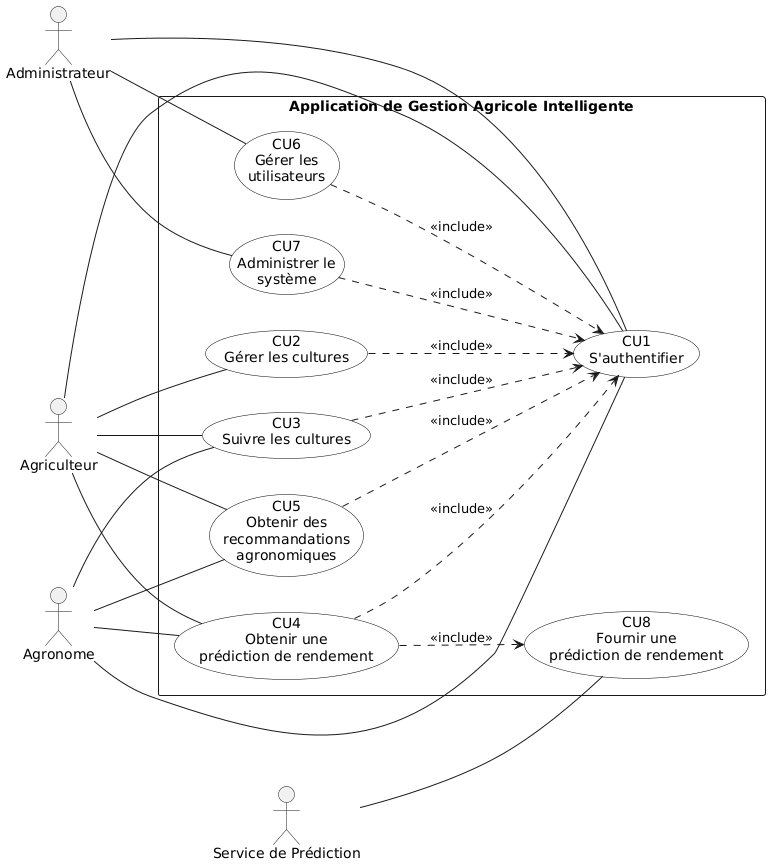
\includegraphics[width=\linewidth]{media/image1.png}
  \caption{Diagramme de cas d'utilisation de l'application de gestion agricole intelligente.}
\end{figure}

\hypertarget{conclusion}{%
\section{Conclusion}\label{conclusion}}

Le diagramme de cas d'utilisation permet de visualiser les interactions
entre les différents acteurs et le système.

Il constitue une représentation synthétique des besoins fonctionnels
exprimés dans le cahier des charges et servira de base à la description
détaillée des cas d'utilisation ainsi qu'à l'élaboration des diagrammes
de séquence système.

\hypertarget{chapitre-6-description-duxe9tailluxe9e-des-cas-dutilisation}{%
\chapter{DESCRIPTION DÉTAILLÉE DES CAS
D'UTILISATION}\label{chapitre-6-description-duxe9tailluxe9e-des-cas-dutilisation}}

\hypertarget{cas-dutilisation-cu1-sauthentifier}{%
\section{Cas d'Utilisation CU1 :
S'authentifier}\label{cas-dutilisation-cu1-sauthentifier}}

\begin{longtable}{@{}p{0.18\linewidth}p{0.78\linewidth}@{}}
\toprule
\rowcolors{2}{gray!10}{white}
\textbf{Élément} & \textbf{Description} \\
\midrule
\endhead
\textbf{Identifiant} & CU1 \\
\textbf{Nom} & S'authentifier \\
\textbf{Objectif} & Permettre à un utilisateur autorisé d'accéder aux
fonctionnalités du système en vérifiant son identité. \\
\textbf{Acteur principal} & Agriculteur, Agronome, Administrateur \\
\textbf{Acteur secondaire} & Aucun \\
\textbf{Préconditions} & L'utilisateur possède un compte valide et le
système est disponible. \\
\textbf{Postconditions} & L'utilisateur est authentifié et accède aux
fonctionnalités correspondant à son profil. \\
\textbf{Déclencheur} & L'utilisateur souhaite accéder au système. \\
\textbf{Priorité} & Critique \\
\textbf{Fréquence d'utilisation} & Élevée \\
\bottomrule
\end{longtable}

\hypertarget{scuxe9nario-nominal}{%
\subsection{Scénario Nominal}\label{scuxe9nario-nominal}}

\begin{longtable}{@{}p{0.18\linewidth}p{0.78\linewidth}@{}}
\toprule
\rowcolors{2}{gray!10}{white}
\textbf{N°} & \textbf{Description} \\
\midrule
\endhead
1 & L'utilisateur demande l'accès au système. \\
2 & Le système invite l'utilisateur à saisir ses informations
d'authentification. \\
3 & L'utilisateur saisit ses informations d'authentification. \\
4 & Le système vérifie les informations fournies. \\
5 & Le système confirme l'authentification. \\
6 & Le système accorde l'accès aux fonctionnalités correspondant au
profil de l'utilisateur. \\
\bottomrule
\end{longtable}

\hypertarget{scuxe9narios-alternatifs}{%
\subsection{Scénarios Alternatifs}\label{scuxe9narios-alternatifs}}

\hypertarget{sa1-informations-dauthentification-incorrectes}{%
\subsubsection{SA1 : Informations d'authentification
incorrectes}\label{sa1-informations-dauthentification-incorrectes}}

\begin{longtable}{@{}p{0.18\linewidth}p{0.78\linewidth}@{}}
\toprule
\rowcolors{2}{gray!10}{white}
\textbf{N°} & \textbf{Description} \\
\midrule
\endhead
4a & Les informations fournies sont invalides. \\
4a1 & Le système informe l'utilisateur que l'authentification a
échoué. \\
4a2 & Le système invite l'utilisateur à saisir de nouvelles
informations. \\
4a3 & Retour à l'étape 2 du scénario nominal. \\
\bottomrule
\end{longtable}

\hypertarget{sa2-compte-inexistant}{%
\subsubsection{SA2 : Compte inexistant}\label{sa2-compte-inexistant}}

\begin{longtable}{@{}p{0.18\linewidth}p{0.78\linewidth}@{}}
\toprule
\rowcolors{2}{gray!10}{white}
\textbf{N°} & \textbf{Description} \\
\midrule
\endhead
4b & Aucun compte correspondant aux informations fournies n'est
trouvé. \\
4b1 & Le système informe l'utilisateur que le compte est introuvable. \\
4b2 & Fin du cas d'utilisation. \\
\bottomrule
\end{longtable}

\hypertarget{sa3-systuxe8me-indisponible}{%
\subsubsection{SA3 : Système
indisponible}\label{sa3-systuxe8me-indisponible}}

\begin{longtable}{@{}p{0.18\linewidth}p{0.78\linewidth}@{}}
\toprule
\rowcolors{2}{gray!10}{white}
\textbf{N°} & \textbf{Description} \\
\midrule
\endhead
4c & Le système ne peut pas effectuer la vérification. \\
4c1 & Le système informe l'utilisateur de l'indisponibilité du
service. \\
4c2 & Fin du cas d'utilisation. \\
\bottomrule
\end{longtable}

\hypertarget{exigences-fonctionnelles-associuxe9es}{%
\subsection{Exigences Fonctionnelles
Associées}\label{exigences-fonctionnelles-associuxe9es}}

\begin{itemize}
\item
  \begin{quote}
  Gestion des comptes utilisateurs.
  \end{quote}
\item
  \begin{quote}
  Authentification des utilisateurs.
  \end{quote}
\end{itemize}

\hypertarget{cas-dutilisation-cu2-guxe9rer-les-cultures}{%
\section{Cas d'Utilisation CU2 : Gérer les
Cultures}\label{cas-dutilisation-cu2-guxe9rer-les-cultures}}

\begin{longtable}{@{}p{0.18\linewidth}p{0.78\linewidth}@{}}
\toprule
\rowcolors{2}{gray!10}{white}
\textbf{Élément} & \textbf{Description} \\
\midrule
\endhead
\textbf{Identifiant} & CU2 \\
\textbf{Nom} & Gérer les cultures \\
\textbf{Objectif} & Permettre à l'agriculteur de gérer les informations
relatives à ses cultures. \\
\textbf{Acteur principal} & Agriculteur \\
\textbf{Acteur secondaire} & Aucun \\
\textbf{Préconditions} & L'agriculteur est authentifié. \\
\textbf{Postconditions} & Les informations relatives aux cultures sont
mises à jour conformément à l'opération effectuée. \\
\textbf{Déclencheur} & L'agriculteur souhaite gérer une culture. \\
\textbf{Priorité} & Critique \\
\textbf{Fréquence d'utilisation} & Élevée \\
\bottomrule
\end{longtable}

\hypertarget{description}{%
\subsection{Description}\label{description}}

Le cas d'utilisation « Gérer les cultures » regroupe l'ensemble des
opérations relatives à la gestion des cultures, notamment :

\begin{itemize}
\item
  \begin{quote}
  l'enregistrement d'une culture ;
  \end{quote}
\item
  \begin{quote}
  la consultation d'une culture ;
  \end{quote}
\item
  \begin{quote}
  la modification d'une culture ;
  \end{quote}
\item
  \begin{quote}
  la suppression d'une culture.
  \end{quote}
\end{itemize}

\hypertarget{scuxe9nario-nominal-1}{%
\subsection{Scénario Nominal}\label{scuxe9nario-nominal-1}}

\begin{longtable}{@{}p{0.18\linewidth}p{0.78\linewidth}@{}}
\toprule
\rowcolors{2}{gray!10}{white}
\textbf{N°} & \textbf{Description} \\
\midrule
\endhead
1 & L'agriculteur sélectionne la fonctionnalité de gestion des
cultures. \\
2 & Le système présente les opérations disponibles. \\
3 & L'agriculteur choisit une opération à effectuer. \\
4 & Le système demande les informations nécessaires à l'opération
choisie. \\
5 & L'agriculteur fournit les informations demandées. \\
6 & Le système traite l'opération demandée. \\
7 & Le système confirme la réussite de l'opération. \\
\bottomrule
\end{longtable}

\hypertarget{scuxe9narios-alternatifs-1}{%
\subsection{Scénarios Alternatifs}\label{scuxe9narios-alternatifs-1}}

\hypertarget{sa1-informations-incompluxe8tes}{%
\subsubsection{SA1 : Informations
incomplètes}\label{sa1-informations-incompluxe8tes}}

\begin{longtable}{@{}p{0.18\linewidth}p{0.78\linewidth}@{}}
\toprule
\rowcolors{2}{gray!10}{white}
\textbf{N°} & \textbf{Description} \\
\midrule
\endhead
5a & Les informations fournies sont incomplètes ou invalides. \\
5a1 & Le système informe l'utilisateur des erreurs détectées. \\
5a2 & Le système demande une correction des informations. \\
5a3 & Retour à l'étape 4 du scénario nominal. \\
\bottomrule
\end{longtable}

\hypertarget{sa2-culture-inexistante}{%
\subsubsection{SA2 : Culture
inexistante}\label{sa2-culture-inexistante}}

\begin{longtable}{@{}p{0.18\linewidth}p{0.78\linewidth}@{}}
\toprule
\rowcolors{2}{gray!10}{white}
\textbf{N°} & \textbf{Description} \\
\midrule
\endhead
6a & La culture concernée n'existe pas. \\
6a1 & Le système informe l'utilisateur que la culture est
introuvable. \\
6a2 & Fin du cas d'utilisation. \\
\bottomrule
\end{longtable}

\hypertarget{sa3-annulation-de-lopuxe9ration}{%
\subsubsection{SA3 : Annulation de
l'opération}\label{sa3-annulation-de-lopuxe9ration}}

\begin{longtable}{@{}p{0.18\linewidth}p{0.78\linewidth}@{}}
\toprule
\rowcolors{2}{gray!10}{white}
\textbf{N°} & \textbf{Description} \\
\midrule
\endhead
3a & L'utilisateur annule l'opération en cours. \\
3a1 & Le système abandonne le traitement demandé. \\
3a2 & Fin du cas d'utilisation. \\
\bottomrule
\end{longtable}

\hypertarget{exigences-fonctionnelles-associuxe9es-1}{%
\subsection{Exigences Fonctionnelles
Associées}\label{exigences-fonctionnelles-associuxe9es-1}}

\begin{itemize}
\item
  \begin{quote}
  Gestion des cultures.
  \end{quote}
\item
  \begin{quote}
  Consultation des cultures.
  \end{quote}
\item
  \begin{quote}
  Modification des cultures.
  \end{quote}
\item
  \begin{quote}
  Suppression des cultures.
  \end{quote}
\end{itemize}

\hypertarget{cas-dutilisation-cu3-suivre-les-cultures}{%
\section{Cas d'Utilisation CU3 : Suivre les
Cultures}\label{cas-dutilisation-cu3-suivre-les-cultures}}

\begin{longtable}{@{}p{0.18\linewidth}p{0.78\linewidth}@{}}
\toprule
\rowcolors{2}{gray!10}{white}
\textbf{Élément} & \textbf{Description} \\
\midrule
\endhead
\textbf{Identifiant} & CU3 \\
\textbf{Nom} & Suivre les cultures \\
\textbf{Objectif} & Permettre à l'utilisateur d'assurer le suivi de
l'évolution des cultures à travers l'enregistrement et la consultation
des observations agricoles. \\
\textbf{Acteur principal} & Agriculteur \\
\textbf{Acteur secondaire} & Agronome \\
\textbf{Préconditions} & L'utilisateur est authentifié et au moins une
culture est enregistrée dans le système. \\
\textbf{Postconditions} & Les observations sont enregistrées ou
consultées et le suivi de la culture est mis à jour. \\
\textbf{Déclencheur} & L'utilisateur souhaite consulter ou enregistrer
des informations relatives à l'évolution d'une culture. \\
\textbf{Priorité} & Critique \\
\textbf{Fréquence d'utilisation} & Élevée \\
\bottomrule
\end{longtable}

\hypertarget{description-1}{%
\subsection{Description}\label{description-1}}

Le cas d'utilisation « Suivre les cultures » permet d'assurer le suivi
de l'évolution des cultures au cours de leur cycle de production.

Il couvre notamment :

\begin{itemize}
\item
  \begin{quote}
  l'enregistrement des observations agricoles ;
  \end{quote}
\item
  \begin{quote}
  la consultation des observations ;
  \end{quote}
\item
  \begin{quote}
  le suivi de l'évolution des cultures.
  \end{quote}
\end{itemize}

\hypertarget{scuxe9nario-nominal-2}{%
\subsection{Scénario Nominal}\label{scuxe9nario-nominal-2}}

\begin{longtable}{@{}p{0.18\linewidth}p{0.78\linewidth}@{}}
\toprule
\rowcolors{2}{gray!10}{white}
\textbf{N°} & \textbf{Description} \\
\midrule
\endhead
1 & L'utilisateur sélectionne une culture à suivre. \\
2 & Le système affiche les informations relatives à la culture
sélectionnée. \\
3 & L'utilisateur demande l'enregistrement ou la consultation
d'observations. \\
4 & Le système présente les informations disponibles ou demande les
nouvelles observations. \\
5 & L'utilisateur consulte les informations ou saisit les observations
demandées. \\
6 & Le système met à jour les informations de suivi de la culture. \\
7 & Le système confirme la réussite de l'opération. \\
\bottomrule
\end{longtable}

\hypertarget{scuxe9narios-alternatifs-2}{%
\subsection{Scénarios Alternatifs}\label{scuxe9narios-alternatifs-2}}

\hypertarget{sa1-culture-inexistante}{%
\subsubsection{SA1 : Culture
inexistante}\label{sa1-culture-inexistante}}

\begin{longtable}{@{}p{0.18\linewidth}p{0.78\linewidth}@{}}
\toprule
\rowcolors{2}{gray!10}{white}
\textbf{N°} & \textbf{Description} \\
\midrule
\endhead
2a & La culture sélectionnée est introuvable. \\
2a1 & Le système informe l'utilisateur que la culture n'existe pas. \\
2a2 & Fin du cas d'utilisation. \\
\bottomrule
\end{longtable}

\hypertarget{sa2-informations-dobservation-invalides}{%
\subsubsection{SA2 : Informations d'observation
invalides}\label{sa2-informations-dobservation-invalides}}

\begin{longtable}{@{}p{0.18\linewidth}p{0.78\linewidth}@{}}
\toprule
\rowcolors{2}{gray!10}{white}
\textbf{N°} & \textbf{Description} \\
\midrule
\endhead
5a & Les informations saisies sont invalides ou incomplètes. \\
5a1 & Le système signale les erreurs détectées. \\
5a2 & Le système demande la correction des informations. \\
5a3 & Retour à l'étape 4 du scénario nominal. \\
\bottomrule
\end{longtable}

\hypertarget{sa3-annulation-de-lopuxe9ration-1}{%
\subsubsection{SA3 : Annulation de
l'opération}\label{sa3-annulation-de-lopuxe9ration-1}}

\begin{longtable}{@{}p{0.18\linewidth}p{0.78\linewidth}@{}}
\toprule
\rowcolors{2}{gray!10}{white}
\textbf{N°} & \textbf{Description} \\
\midrule
\endhead
3a & L'utilisateur annule l'opération. \\
3a1 & Le système abandonne l'opération en cours. \\
3a2 & Fin du cas d'utilisation. \\
\bottomrule
\end{longtable}

\hypertarget{exigences-fonctionnelles-associuxe9es-2}{%
\subsection{Exigences Fonctionnelles
Associées}\label{exigences-fonctionnelles-associuxe9es-2}}

\begin{itemize}
\item
  \begin{quote}
  Enregistrement des observations agricoles.
  \end{quote}
\item
  \begin{quote}
  Consultation des observations.
  \end{quote}
\item
  \begin{quote}
  Suivi de l'évolution des cultures.
  \end{quote}
\end{itemize}

\hypertarget{cas-dutilisation-cu4-obtenir-une-pruxe9diction-de-rendement}{%
\section{Cas d'Utilisation CU4 : Obtenir une Prédiction de
Rendement}\label{cas-dutilisation-cu4-obtenir-une-pruxe9diction-de-rendement}}

\begin{longtable}{@{}p{0.18\linewidth}p{0.78\linewidth}@{}}
\toprule
\rowcolors{2}{gray!10}{white}
\textbf{Élément} & \textbf{Description} \\
\midrule
\endhead
\textbf{Identifiant} & CU4 \\
\textbf{Nom} & Obtenir une prédiction de rendement \\
\textbf{Objectif} & Permettre à l'utilisateur d'obtenir une estimation
du rendement attendu pour une culture. \\
\textbf{Acteur principal} & Agriculteur \\
\textbf{Acteur secondaire} & Agronome \\
\textbf{Acteur externe} & Service de Prédiction \\
\textbf{Préconditions} & L'utilisateur est authentifié et une culture
est disponible pour l'analyse. \\
\textbf{Postconditions} & Une estimation de rendement est fournie à
l'utilisateur. \\
\textbf{Déclencheur} & L'utilisateur souhaite connaître le rendement
prévisionnel d'une culture. \\
\textbf{Priorité} & Critique \\
\textbf{Fréquence d'utilisation} & Moyenne \\
\bottomrule
\end{longtable}

\hypertarget{description-2}{%
\subsection{Description}\label{description-2}}

Le cas d'utilisation « Obtenir une prédiction de rendement » permet
d'estimer le rendement futur d'une culture à partir des informations
disponibles dans le système.

Cette fonctionnalité constitue une aide à la décision pour les
utilisateurs.

\hypertarget{scuxe9nario-nominal-3}{%
\subsection{Scénario Nominal}\label{scuxe9nario-nominal-3}}

\begin{longtable}{@{}p{0.18\linewidth}p{0.78\linewidth}@{}}
\toprule
\rowcolors{2}{gray!10}{white}
\textbf{N°} & \textbf{Description} \\
\midrule
\endhead
1 & L'utilisateur sélectionne une culture. \\
2 & L'utilisateur demande une prédiction de rendement. \\
3 & Le système prépare les informations nécessaires à l'analyse. \\
4 & Le système sollicite le service de prédiction. \\
5 & Le service de prédiction fournit une estimation du rendement. \\
6 & Le système présente le résultat de la prédiction à l'utilisateur. \\
7 & L'utilisateur consulte le résultat obtenu. \\
\bottomrule
\end{longtable}

\hypertarget{scuxe9narios-alternatifs-3}{%
\subsection{Scénarios Alternatifs}\label{scuxe9narios-alternatifs-3}}

\hypertarget{sa1-culture-inexistante-1}{%
\subsubsection{SA1 : Culture
inexistante}\label{sa1-culture-inexistante-1}}

\begin{longtable}{@{}p{0.18\linewidth}p{0.78\linewidth}@{}}
\toprule
\rowcolors{2}{gray!10}{white}
\textbf{N°} & \textbf{Description} \\
\midrule
\endhead
1a & La culture sélectionnée est introuvable. \\
1a1 & Le système informe l'utilisateur que la culture n'existe pas. \\
1a2 & Fin du cas d'utilisation. \\
\bottomrule
\end{longtable}

\hypertarget{sa2-uxe9chec-de-la-pruxe9diction}{%
\subsubsection{SA2 : Échec de la
prédiction}\label{sa2-uxe9chec-de-la-pruxe9diction}}

\begin{longtable}{@{}p{0.18\linewidth}p{0.78\linewidth}@{}}
\toprule
\rowcolors{2}{gray!10}{white}
\textbf{N°} & \textbf{Description} \\
\midrule
\endhead
5a & Le service de prédiction ne fournit aucun résultat. \\
5a1 & Le système informe l'utilisateur de l'échec de la prédiction. \\
5a2 & Fin du cas d'utilisation. \\
\bottomrule
\end{longtable}

\hypertarget{sa3-donnuxe9es-insuffisantes}{%
\subsubsection{SA3 : Données
insuffisantes}\label{sa3-donnuxe9es-insuffisantes}}

\begin{longtable}{@{}p{0.18\linewidth}p{0.78\linewidth}@{}}
\toprule
\rowcolors{2}{gray!10}{white}
\textbf{N°} & \textbf{Description} \\
\midrule
\endhead
3a & Les informations disponibles sont insuffisantes pour effectuer une
prédiction. \\
3a1 & Le système informe l'utilisateur que les données sont
insuffisantes. \\
3a2 & Fin du cas d'utilisation. \\
\bottomrule
\end{longtable}

\hypertarget{exigences-fonctionnelles-associuxe9es-3}{%
\subsection{Exigences Fonctionnelles
Associées}\label{exigences-fonctionnelles-associuxe9es-3}}

\begin{itemize}
\item
  \begin{quote}
  Demande de prédiction de rendement.
  \end{quote}
\item
  \begin{quote}
  Consultation des résultats de prédiction.
  \end{quote}
\item
  \begin{quote}
  Assistance à la décision agricole.
  \end{quote}
\end{itemize}

\hypertarget{cas-dutilisation-cu5-obtenir-des-recommandations-agronomiques}{%
\section{Cas d'Utilisation CU5 : Obtenir des Recommandations
Agronomiques}\label{cas-dutilisation-cu5-obtenir-des-recommandations-agronomiques}}

\begin{longtable}{@{}p{0.18\linewidth}p{0.78\linewidth}@{}}
\toprule
\rowcolors{2}{gray!10}{white}
\textbf{Élément} & \textbf{Description} \\
\midrule
\endhead
\textbf{Identifiant} & CU5 \\
\textbf{Nom} & Obtenir des recommandations agronomiques \\
\textbf{Objectif} & Permettre à l'utilisateur d'obtenir des
recommandations adaptées à la situation d'une culture afin d'améliorer
la prise de décision agricole. \\
\textbf{Acteur principal} & Agriculteur \\
\textbf{Acteur secondaire} & Agronome \\
\textbf{Préconditions} & L'utilisateur est authentifié et au moins une
culture est enregistrée dans le système. \\
\textbf{Postconditions} & Les recommandations agronomiques sont mises à
disposition de l'utilisateur. \\
\textbf{Déclencheur} & L'utilisateur souhaite obtenir des conseils ou
recommandations concernant une culture. \\
\textbf{Priorité} & Critique \\
\textbf{Fréquence d'utilisation} & Moyenne \\
\bottomrule
\end{longtable}

\hypertarget{description-3}{%
\subsection{Description}\label{description-3}}

Le cas d'utilisation « Obtenir des recommandations agronomiques » permet
de fournir à l'utilisateur des conseils adaptés à la situation observée
sur une culture.

Les recommandations peuvent concerner :

\begin{itemize}
\item
  \begin{quote}
  le suivi de la culture ;
  \end{quote}
\item
  \begin{quote}
  les actions à entreprendre ;
  \end{quote}
\item
  \begin{quote}
  l'amélioration des pratiques agricoles.
  \end{quote}
\end{itemize}

\hypertarget{scuxe9nario-nominal-4}{%
\subsection{Scénario Nominal}\label{scuxe9nario-nominal-4}}

\begin{longtable}{@{}p{0.18\linewidth}p{0.78\linewidth}@{}}
\toprule
\rowcolors{2}{gray!10}{white}
\textbf{N°} & \textbf{Description} \\
\midrule
\endhead
1 & L'utilisateur sélectionne une culture. \\
2 & L'utilisateur demande des recommandations agronomiques. \\
3 & Le système analyse les informations disponibles relatives à la
culture. \\
4 & Le système détermine les recommandations appropriées. \\
5 & Le système présente les recommandations à l'utilisateur. \\
6 & L'utilisateur consulte les recommandations proposées. \\
\bottomrule
\end{longtable}

\hypertarget{scuxe9narios-alternatifs-4}{%
\subsection{Scénarios Alternatifs}\label{scuxe9narios-alternatifs-4}}

\hypertarget{sa1-culture-inexistante-2}{%
\subsubsection{SA1 : Culture
inexistante}\label{sa1-culture-inexistante-2}}

\begin{longtable}{@{}p{0.18\linewidth}p{0.78\linewidth}@{}}
\toprule
\rowcolors{2}{gray!10}{white}
\textbf{N°} & \textbf{Description} \\
\midrule
\endhead
1a & La culture sélectionnée est introuvable. \\
1a1 & Le système informe l'utilisateur que la culture n'existe pas. \\
1a2 & Fin du cas d'utilisation. \\
\bottomrule
\end{longtable}

\hypertarget{sa2-donnuxe9es-insuffisantes}{%
\subsubsection{SA2 : Données
insuffisantes}\label{sa2-donnuxe9es-insuffisantes}}

\begin{longtable}{@{}p{0.18\linewidth}p{0.78\linewidth}@{}}
\toprule
\rowcolors{2}{gray!10}{white}
\textbf{N°} & \textbf{Description} \\
\midrule
\endhead
3a & Les informations disponibles sont insuffisantes pour produire des
recommandations pertinentes. \\
3a1 & Le système informe l'utilisateur que les données sont
insuffisantes. \\
3a2 & Fin du cas d'utilisation. \\
\bottomrule
\end{longtable}

\hypertarget{sa3-aucune-recommandation-disponible}{%
\subsubsection{SA3 : Aucune recommandation
disponible}\label{sa3-aucune-recommandation-disponible}}

\begin{longtable}{@{}p{0.18\linewidth}p{0.78\linewidth}@{}}
\toprule
\rowcolors{2}{gray!10}{white}
\textbf{N°} & \textbf{Description} \\
\midrule
\endhead
4a & Aucune recommandation n'est disponible pour la situation
analysée. \\
4a1 & Le système informe l'utilisateur qu'aucune recommandation ne peut
être proposée. \\
4a2 & Fin du cas d'utilisation. \\
\bottomrule
\end{longtable}

\hypertarget{exigences-fonctionnelles-associuxe9es-4}{%
\subsection{Exigences Fonctionnelles
Associées}\label{exigences-fonctionnelles-associuxe9es-4}}

\begin{itemize}
\item
  \begin{quote}
  Génération de recommandations agronomiques.
  \end{quote}
\item
  \begin{quote}
  Consultation des recommandations.
  \end{quote}
\item
  \begin{quote}
  Assistance à la décision agricole.
  \end{quote}
\end{itemize}

\hypertarget{cas-dutilisation-cu6-guxe9rer-les-utilisateurs}{%
\section{Cas d'Utilisation CU6 : Gérer les
Utilisateurs}\label{cas-dutilisation-cu6-guxe9rer-les-utilisateurs}}

\begin{longtable}{@{}p{0.18\linewidth}p{0.78\linewidth}@{}}
\toprule
\rowcolors{2}{gray!10}{white}
\textbf{Élément} & \textbf{Description} \\
\midrule
\endhead
\textbf{Identifiant} & CU6 \\
\textbf{Nom} & Gérer les utilisateurs \\
\textbf{Objectif} & Permettre à l'administrateur de gérer les comptes
utilisateurs du système. \\
\textbf{Acteur principal} & Administrateur \\
\textbf{Acteur secondaire} & Aucun \\
\textbf{Préconditions} & L'administrateur est authentifié. \\
\textbf{Postconditions} & Les informations relatives aux utilisateurs
sont mises à jour conformément à l'opération effectuée. \\
\textbf{Déclencheur} & L'administrateur souhaite effectuer une opération
sur un compte utilisateur. \\
\textbf{Priorité} & Critique \\
\textbf{Fréquence d'utilisation} & Moyenne \\
\bottomrule
\end{longtable}

\hypertarget{description-4}{%
\subsection{Description}\label{description-4}}

Le cas d'utilisation « Gérer les utilisateurs » permet à
l'administrateur d'assurer la gestion des comptes utilisateurs du
système.

Il couvre notamment :

\begin{itemize}
\item
  \begin{quote}
  la création de comptes utilisateurs ;
  \end{quote}
\item
  \begin{quote}
  la consultation des informations d'un utilisateur ;
  \end{quote}
\item
  \begin{quote}
  la modification des informations d'un utilisateur ;
  \end{quote}
\item
  \begin{quote}
  la suppression d'un utilisateur.
  \end{quote}
\end{itemize}

\hypertarget{scuxe9nario-nominal-5}{%
\subsection{Scénario Nominal}\label{scuxe9nario-nominal-5}}

\begin{longtable}{@{}p{0.18\linewidth}p{0.78\linewidth}@{}}
\toprule
\rowcolors{2}{gray!10}{white}
\textbf{N°} & \textbf{Description} \\
\midrule
\endhead
1 & L'administrateur accède à la gestion des utilisateurs. \\
2 & Le système présente les opérations disponibles. \\
3 & L'administrateur sélectionne une opération. \\
4 & Le système demande les informations nécessaires. \\
5 & L'administrateur fournit les informations demandées. \\
6 & Le système exécute l'opération demandée. \\
7 & Le système confirme la réussite de l'opération. \\
\bottomrule
\end{longtable}

\hypertarget{scuxe9narios-alternatifs-5}{%
\subsection{Scénarios Alternatifs}\label{scuxe9narios-alternatifs-5}}

\hypertarget{sa1-informations-invalides}{%
\subsubsection{SA1 : Informations
invalides}\label{sa1-informations-invalides}}

\begin{longtable}{@{}p{0.18\linewidth}p{0.78\linewidth}@{}}
\toprule
\rowcolors{2}{gray!10}{white}
\textbf{N°} & \textbf{Description} \\
\midrule
\endhead
5a & Les informations fournies sont invalides ou incomplètes. \\
5a1 & Le système informe l'administrateur des erreurs détectées. \\
5a2 & Le système demande une correction des informations. \\
5a3 & Retour à l'étape 4 du scénario nominal. \\
\bottomrule
\end{longtable}

\hypertarget{sa2-utilisateur-introuvable}{%
\subsubsection{SA2 : Utilisateur
introuvable}\label{sa2-utilisateur-introuvable}}

\begin{longtable}{@{}p{0.18\linewidth}p{0.78\linewidth}@{}}
\toprule
\rowcolors{2}{gray!10}{white}
\textbf{N°} & \textbf{Description} \\
\midrule
\endhead
6a & L'utilisateur concerné n'existe pas. \\
6a1 & Le système informe l'administrateur que l'utilisateur est
introuvable. \\
6a2 & Fin du cas d'utilisation. \\
\bottomrule
\end{longtable}

\hypertarget{sa3-annulation-de-lopuxe9ration-2}{%
\subsubsection{SA3 : Annulation de
l'opération}\label{sa3-annulation-de-lopuxe9ration-2}}

\begin{longtable}{@{}p{0.18\linewidth}p{0.78\linewidth}@{}}
\toprule
\rowcolors{2}{gray!10}{white}
\textbf{N°} & \textbf{Description} \\
\midrule
\endhead
3a & L'administrateur annule l'opération en cours. \\
3a1 & Le système abandonne l'opération demandée. \\
3a2 & Fin du cas d'utilisation. \\
\bottomrule
\end{longtable}

\hypertarget{exigences-fonctionnelles-associuxe9es-5}{%
\subsection{Exigences Fonctionnelles
Associées}\label{exigences-fonctionnelles-associuxe9es-5}}

\begin{itemize}
\item
  \begin{quote}
  Gestion des comptes utilisateurs.
  \end{quote}
\item
  \begin{quote}
  Administration des utilisateurs.
  \end{quote}
\end{itemize}

\hypertarget{cas-dutilisation-cu7-administrer-le-systuxe8me}{%
\section{Cas d'Utilisation CU7 : Administrer le
Système}\label{cas-dutilisation-cu7-administrer-le-systuxe8me}}

\begin{longtable}{@{}p{0.18\linewidth}p{0.78\linewidth}@{}}
\toprule
\rowcolors{2}{gray!10}{white}
\textbf{Élément} & \textbf{Description} \\
\midrule
\endhead
\textbf{Identifiant} & CU7 \\
\textbf{Nom} & Administrer le système \\
\textbf{Objectif} & Permettre à l'administrateur d'assurer le bon
fonctionnement général de l'application. \\
\textbf{Acteur principal} & Administrateur \\
\textbf{Acteur secondaire} & Aucun \\
\textbf{Préconditions} & L'administrateur est authentifié. \\
\textbf{Postconditions} & Les opérations d'administration sont réalisées
avec succès et le système reste opérationnel. \\
\textbf{Déclencheur} & L'administrateur souhaite effectuer une opération
d'administration. \\
\textbf{Priorité} & Élevée \\
\textbf{Fréquence d'utilisation} & Faible à moyenne \\
\bottomrule
\end{longtable}

\hypertarget{description-5}{%
\subsection{Description}\label{description-5}}

Le cas d'utilisation « Administrer le système » permet à
l'administrateur d'assurer la gestion générale de la plateforme.

Il couvre notamment :

\begin{itemize}
\item
  \begin{quote}
  la consultation des informations globales du système ;
  \end{quote}
\item
  \begin{quote}
  la supervision du fonctionnement général ;
  \end{quote}
\item
  \begin{quote}
  l'administration des données de référence ;
  \end{quote}
\item
  \begin{quote}
  les opérations nécessaires au bon fonctionnement de la plateforme.
  \end{quote}
\end{itemize}

\hypertarget{scuxe9nario-nominal-6}{%
\subsection{Scénario Nominal}\label{scuxe9nario-nominal-6}}

\begin{longtable}{@{}p{0.18\linewidth}p{0.78\linewidth}@{}}
\toprule
\rowcolors{2}{gray!10}{white}
\textbf{N°} & \textbf{Description} \\
\midrule
\endhead
1 & L'administrateur accède aux fonctionnalités d'administration. \\
2 & Le système présente les opérations d'administration disponibles. \\
3 & L'administrateur sélectionne une opération. \\
4 & Le système demande les informations nécessaires à l'opération. \\
5 & L'administrateur fournit les informations demandées. \\
6 & Le système exécute l'opération d'administration. \\
7 & Le système confirme la réussite de l'opération. \\
\bottomrule
\end{longtable}

\hypertarget{scuxe9narios-alternatifs-6}{%
\subsection{Scénarios Alternatifs}\label{scuxe9narios-alternatifs-6}}

\hypertarget{sa1-informations-invalides-1}{%
\subsubsection{SA1 : Informations
invalides}\label{sa1-informations-invalides-1}}

\begin{longtable}{@{}p{0.18\linewidth}p{0.78\linewidth}@{}}
\toprule
\rowcolors{2}{gray!10}{white}
\textbf{N°} & \textbf{Description} \\
\midrule
\endhead
5a & Les informations fournies sont invalides ou incomplètes. \\
5a1 & Le système informe l'administrateur des erreurs détectées. \\
5a2 & Le système demande une correction des informations. \\
5a3 & Retour à l'étape 4 du scénario nominal. \\
\bottomrule
\end{longtable}

\hypertarget{sa2-opuxe9ration-impossible}{%
\subsubsection{SA2 : Opération
impossible}\label{sa2-opuxe9ration-impossible}}

\begin{longtable}{@{}p{0.18\linewidth}p{0.78\linewidth}@{}}
\toprule
\rowcolors{2}{gray!10}{white}
\textbf{N°} & \textbf{Description} \\
\midrule
\endhead
6a & L'opération demandée ne peut pas être exécutée. \\
6a1 & Le système informe l'administrateur de l'échec de l'opération. \\
6a2 & Fin du cas d'utilisation. \\
\bottomrule
\end{longtable}

\hypertarget{sa3-annulation-de-lopuxe9ration-3}{%
\subsubsection{SA3 : Annulation de
l'opération}\label{sa3-annulation-de-lopuxe9ration-3}}

\begin{longtable}{@{}p{0.18\linewidth}p{0.78\linewidth}@{}}
\toprule
\rowcolors{2}{gray!10}{white}
\textbf{N°} & \textbf{Description} \\
\midrule
\endhead
3a & L'administrateur annule l'opération en cours. \\
3a1 & Le système abandonne l'opération demandée. \\
3a2 & Fin du cas d'utilisation. \\
\bottomrule
\end{longtable}

\hypertarget{exigences-fonctionnelles-associuxe9es-6}{%
\subsection{Exigences Fonctionnelles
Associées}\label{exigences-fonctionnelles-associuxe9es-6}}

\begin{itemize}
\item
  \begin{quote}
  Administration du système.
  \end{quote}
\item
  \begin{quote}
  Gestion des données de référence.
  \end{quote}
\item
  \begin{quote}
  Supervision du fonctionnement de la plateforme.
  \end{quote}
\end{itemize}

\hypertarget{cas-dutilisation-cu8-fournir-une-pruxe9diction-de-rendement}{%
\section{Cas d'Utilisation CU8 : Fournir une Prédiction de
Rendement}\label{cas-dutilisation-cu8-fournir-une-pruxe9diction-de-rendement}}

\begin{longtable}{@{}p{0.18\linewidth}p{0.78\linewidth}@{}}
\toprule
\rowcolors{2}{gray!10}{white}
\textbf{Élément} & \textbf{Description} \\
\midrule
\endhead
\textbf{Identifiant} & CU8 \\
\textbf{Nom} & Fournir une prédiction de rendement \\
\textbf{Objectif} & Permettre au service de prédiction de fournir une
estimation du rendement d'une culture à partir des informations
transmises par le système. \\
\textbf{Acteur principal} & Service de Prédiction \\
\textbf{Acteur secondaire} & Aucun \\
\textbf{Préconditions} & Une demande de prédiction a été initiée par le
système dans le cadre du cas d'utilisation CU4. \\
\textbf{Postconditions} & Une estimation de rendement est transmise au
système. \\
\textbf{Déclencheur} & Réception d'une demande de prédiction provenant
du système. \\
\textbf{Priorité} & Élevée \\
\textbf{Fréquence d'utilisation} & Dépend des demandes de prédiction
effectuées par les utilisateurs. \\
\bottomrule
\end{longtable}

\hypertarget{description-6}{%
\subsection{Description}\label{description-6}}

Le cas d'utilisation « Fournir une prédiction de rendement » représente
l'intervention du service externe de prédiction.

Il permet de produire une estimation du rendement attendu d'une culture
à partir des informations fournies par le système.

Ce cas d'utilisation est inclus dans le cas d'utilisation CU4 « Obtenir
une prédiction de rendement ».

\hypertarget{scuxe9nario-nominal-7}{%
\subsection{Scénario Nominal}\label{scuxe9nario-nominal-7}}

\begin{longtable}{@{}p{0.18\linewidth}p{0.78\linewidth}@{}}
\toprule
\rowcolors{2}{gray!10}{white}
\textbf{N°} & \textbf{Description} \\
\midrule
\endhead
1 & Le système transmet les informations nécessaires au service de
prédiction. \\
2 & Le service de prédiction reçoit les informations. \\
3 & Le service analyse les informations reçues. \\
4 & Le service produit une estimation du rendement. \\
5 & Le service transmet le résultat au système. \\
\bottomrule
\end{longtable}

\hypertarget{scuxe9narios-alternatifs-7}{%
\subsection{Scénarios Alternatifs}\label{scuxe9narios-alternatifs-7}}

\hypertarget{sa1-informations-insuffisantes}{%
\subsubsection{SA1 : Informations
insuffisantes}\label{sa1-informations-insuffisantes}}

\begin{longtable}{@{}p{0.18\linewidth}p{0.78\linewidth}@{}}
\toprule
\rowcolors{2}{gray!10}{white}
\textbf{N°} & \textbf{Description} \\
\midrule
\endhead
3a & Les informations reçues sont insuffisantes pour effectuer
l'analyse. \\
3a1 & Le service informe le système de l'impossibilité de produire une
prédiction. \\
3a2 & Fin du cas d'utilisation. \\
\bottomrule
\end{longtable}

\hypertarget{sa2-uxe9chec-du-traitement}{%
\subsubsection{SA2 : Échec du
traitement}\label{sa2-uxe9chec-du-traitement}}

\begin{longtable}{@{}p{0.18\linewidth}p{0.78\linewidth}@{}}
\toprule
\rowcolors{2}{gray!10}{white}
\textbf{N°} & \textbf{Description} \\
\midrule
\endhead
4a & Une erreur survient durant l'analyse. \\
4a1 & Le service informe le système de l'échec du traitement. \\
4a2 & Fin du cas d'utilisation. \\
\bottomrule
\end{longtable}

\hypertarget{exigences-fonctionnelles-associuxe9es-7}{%
\subsection{Exigences Fonctionnelles
Associées}\label{exigences-fonctionnelles-associuxe9es-7}}

\begin{itemize}
\item
  \begin{quote}
  Fourniture des prédictions de rendement.
  \end{quote}
\item
  \begin{quote}
  Assistance au cas d'utilisation CU4 : Obtenir une prédiction de
  rendement.
  \end{quote}
\end{itemize}

\hypertarget{chapitre-7-diagrammes-de-suxe9quence-systuxe8me}{%
\chapter{DIAGRAMMES DE SÉQUENCE
SYSTÈME}\label{chapitre-7-diagrammes-de-suxe9quence-systuxe8me}}

\hypertarget{introduction-3}{%
\section{Introduction}\label{introduction-3}}

Les diagrammes de séquence système permettent de représenter les
interactions entre les acteurs et le système pour la réalisation des
différents cas d'utilisation.

Dans cette phase d'analyse, le système est considéré comme une boîte
noire. Les diagrammes mettent uniquement en évidence les échanges entre
les acteurs et le système sans détailler les mécanismes internes de
traitement.

L'objectif est de décrire le comportement attendu du système à travers
les différents scénarios identifiés lors de l'analyse des besoins.

Les diagrammes présentés dans ce chapitre sont directement dérivés des
descriptions détaillées des cas d'utilisation et constituent une
transition vers la phase de conception.

\hypertarget{diagramme-de-suxe9quence-systuxe8me-du-cas-dutilisation-cu1-sauthentifier}{%
\section{Diagramme de Séquence Système du Cas d'Utilisation CU1 :
S'authentifier}\label{diagramme-de-suxe9quence-systuxe8me-du-cas-dutilisation-cu1-sauthentifier}}

Le diagramme suivant illustre les interactions entre l'utilisateur et le
système lors du processus d'authentification.

\begin{figure}[H]
  \centering
  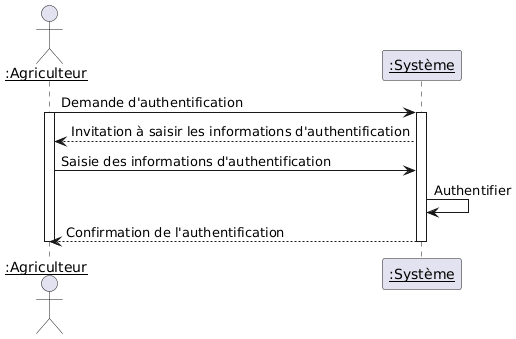
\includegraphics[width=\linewidth]{media/image2.png}
  \caption{Diagramme de séquence système du cas d'utilisation « S'authentifier ».}
\end{figure}

\hypertarget{diagramme-de-suxe9quence-systuxe8me-du-cas-dutilisation-cu2-guxe9rer-les-cultures}{%
\section{Diagramme de Séquence Système du Cas d'Utilisation CU2 :
Gérer les
Cultures}\label{diagramme-de-suxe9quence-systuxe8me-du-cas-dutilisation-cu2-guxe9rer-les-cultures}}

Le diagramme suivant illustre les interactions entre l'agriculteur et le
système lors de la gestion des cultures.

\begin{figure}[H]
  \centering
  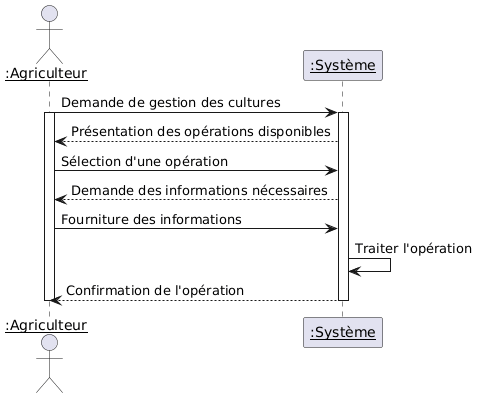
\includegraphics[width=\linewidth]{media/image3.png}
  \caption{Diagramme de séquence système du cas d'utilisation « Gérer les cultures ».}
\end{figure}

\hypertarget{diagramme-de-suxe9quence-systuxe8me-du-cas-dutilisation-cu3-suivre-les-cultures}{%
\section{Diagramme de Séquence Système du Cas d'Utilisation CU3 :
Suivre les
Cultures}\label{diagramme-de-suxe9quence-systuxe8me-du-cas-dutilisation-cu3-suivre-les-cultures}}

Le diagramme suivant illustre les interactions entre l'utilisateur et le
système lors du suivi des cultures.

\begin{figure}[H]
  \centering
  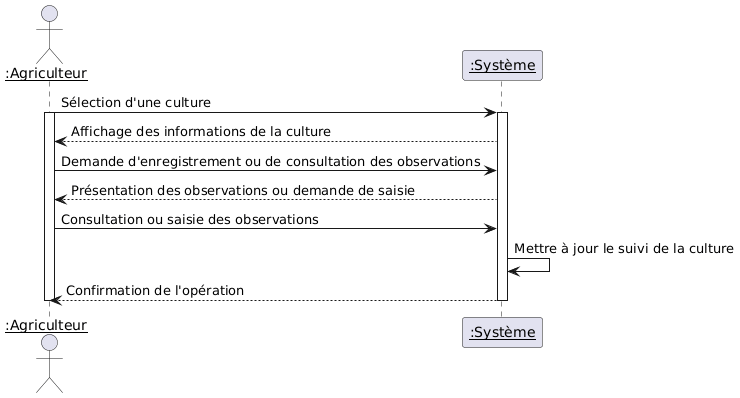
\includegraphics[width=\linewidth]{media/image4.png}
  \caption{Diagramme de séquence système du cas d'utilisation « Suivre les cultures ».}
\end{figure}

\hypertarget{diagramme-de-suxe9quence-systuxe8me-du-cas-dutilisation-cu4-obtenir-une-pruxe9diction-de-rendement}{%
\section{Diagramme de Séquence Système du Cas d'Utilisation CU4 :
Obtenir une Prédiction de
Rendement}\label{diagramme-de-suxe9quence-systuxe8me-du-cas-dutilisation-cu4-obtenir-une-pruxe9diction-de-rendement}}

Le diagramme suivant illustre les interactions entre l'utilisateur et le
système lors de l'obtention d'une prédiction de rendement.

\begin{figure}[H]
  \centering
  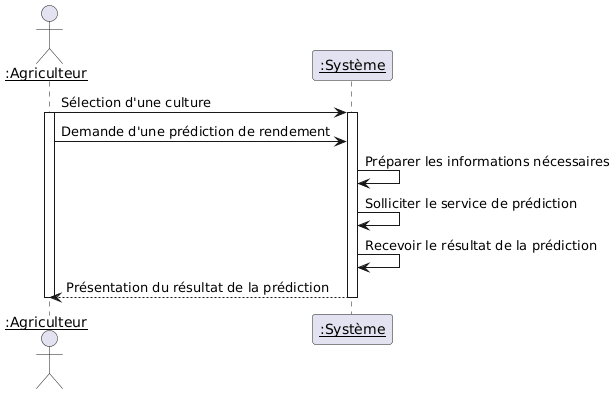
\includegraphics[width=\linewidth]{media/image5.png}
  \caption{Diagramme de séquence système du cas d'utilisation « Obtenir une prédiction de rendement ».}
\end{figure}

\hypertarget{diagramme-de-suxe9quence-systuxe8me-du-cas-dutilisation-cu5-obtenir-des-recommandations-agronomiques}{%
\section{Diagramme de Séquence Système du Cas d'Utilisation CU5 :
Obtenir des Recommandations
Agronomiques}\label{diagramme-de-suxe9quence-systuxe8me-du-cas-dutilisation-cu5-obtenir-des-recommandations-agronomiques}}

Le diagramme suivant illustre les interactions entre l'utilisateur et le
système lors de l'obtention de recommandations agronomiques.

\begin{figure}[H]
  \centering
  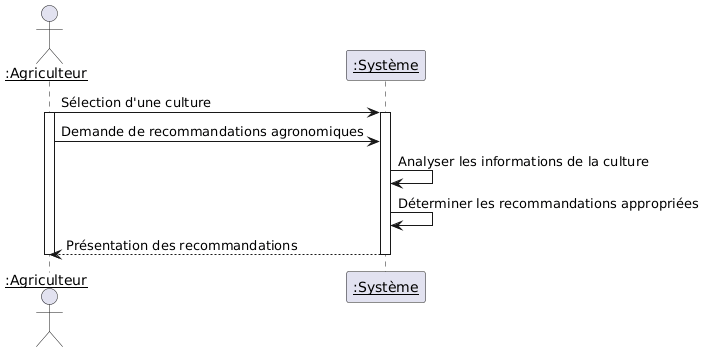
\includegraphics[width=\linewidth]{media/image6.png}
  \caption{Diagramme de séquence système du cas d'utilisation « Obtenir des recommandations agronomiques ».}
\end{figure}

\hypertarget{diagramme-de-suxe9quence-systuxe8me-du-cas-dutilisation-cu6-guxe9rer-les-utilisateurs}{%
\section{Diagramme de Séquence Système du Cas d'Utilisation CU6 :
Gérer les
Utilisateurs}\label{diagramme-de-suxe9quence-systuxe8me-du-cas-dutilisation-cu6-guxe9rer-les-utilisateurs}}

Le diagramme suivant illustre les interactions entre l'administrateur et
le système lors de la gestion des utilisateurs.

\begin{figure}[H]
  \centering
  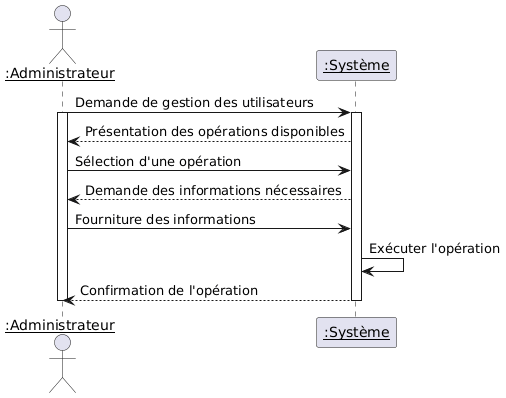
\includegraphics[width=\linewidth]{media/image7.png}
  \caption{Diagramme de séquence système du cas d'utilisation « Gérer les utilisateurs ».}
\end{figure}

\hypertarget{diagramme-de-suxe9quence-systuxe8me-du-cas-dutilisation-cu7-administrer-le-systuxe8me}{%
\section{Diagramme de Séquence Système du Cas d'Utilisation CU7 :
Administrer le
Système}\label{diagramme-de-suxe9quence-systuxe8me-du-cas-dutilisation-cu7-administrer-le-systuxe8me}}

Le diagramme suivant illustre les interactions entre l'administrateur et
le système lors des opérations d'administration.

\begin{figure}[H]
  \centering
  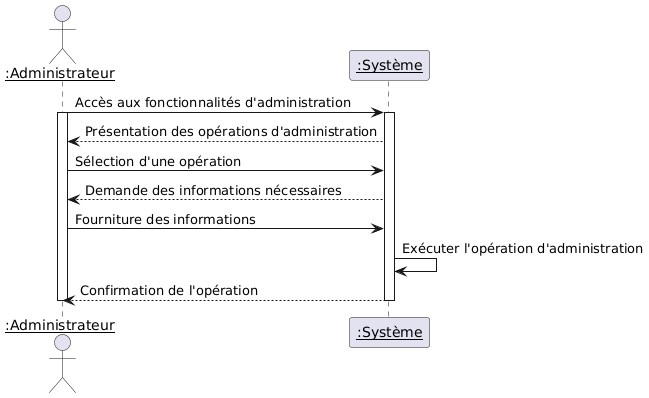
\includegraphics[width=\linewidth]{media/image8.png}
  \caption{Diagramme de séquence système du cas d'utilisation « Administrer le système ».}
\end{figure}

\hypertarget{chapitre-8-conclusion}{%
\chapter{CONCLUSION}\label{chapitre-8-conclusion}}

Le présent cahier d'analyse a permis d'étudier le comportement attendu
de l'application de gestion agricole intelligente à partir des besoins
exprimés dans le cahier des charges.

L'analyse réalisée a conduit à l'identification des différents acteurs
du système ainsi qu'à la définition des principaux services qui leur
sont offerts. Ces services ont été modélisés sous forme de cas
d'utilisation afin de mettre en évidence les interactions entre les
utilisateurs et le système.

Les cas d'utilisation identifiés ont ensuite été décrits de manière
détaillée à travers des scénarios nominaux et alternatifs permettant de
préciser le comportement attendu du système dans différentes situations.

Enfin, les diagrammes de séquence système ont permis de représenter les
échanges entre les acteurs et le système tout en conservant une vision
externe du système conformément aux principes de la phase d'analyse.

Les différents modèles élaborés au cours de cette phase constituent une
base solide pour la conception du système. Ils serviront notamment à
définir l'architecture de la solution, les composants logiciels, les
diagrammes de classes ainsi que les mécanismes internes nécessaires à
l'implémentation de l'application.

Le cahier d'analyse constitue ainsi le lien entre l'expression des
besoins et la conception détaillée de la solution logicielle.

\end{document}
